
\chapter{Control}
\label{cha:control}

As said in the \nameref{cha:background} chapter, a \CIPN{} can be used to
represent the control of a system and then this Petri net can be converted into
a \LD{}, with the aim of being implemented in a \PLC. So, this section will be divided in two
parts: the first part to describe the logic of the control and its design using \CIPN{} and
the second part for the implementation in the \PLC.

\section{Logic}
\label{sec:logic}
The logic of the control is to use the 6 units presented in
\Autoref{cha:system}, to assemble cubes made of a metallic half cube with a
white plastic one on top, and once the cube is assembled it is stored in one of
the store spaces of the \verb|Storage Unit|. 
The logic is divided in 10 modules:
 Initialization, Metal Cube half sorting, Plastic Cube half sorting, Arm From
 Conveyor Belt to Assembly Unit, Assembly Unit, Arm From Assembly Unit to
 Storage Unit, Storage Unit positioning (y axis), Storage Unit positioning (x
 axis), Cube Storage and Arm Stop Logic.

Each module will be briefly described in the next subsections, and their Petri
Nets will be presented along with tables that describe the meaning of each place
and transition.

\begin{observation}
  Each Petri net shown in this chapter is a section of a complete Petri net.
  The complete one is presented in \Autoref{cha:CompletePetriNet}. As said
in \Autoref{cha:background} the dotted places\slash transitions represent places\slash transitions that are part of other sections of the Petri net. In the
digital form of this work, it is possible to travel between figures by clicking
the name of the dotted places\slash transitions. By clicking in normal
places\slash transitions it is possible to travel between the figure and its
corresponding entry in the table that describes its meaning.
  
\end{observation}
\subsection{Initialization}
This module has as objective to make sure that all units are in order to begin
the assembling process, that means, all variables used are reset, the arm is
calibrated, the conveyor belt is free of pieces, all cylinders are retracted,
the assembly unit is ready to receive a piece and the storage unit is in its
rightmost and lower position. The Petri net used for this module can be seen in
\Autoref{fig:petriInitialization} and the corresponding meaning of its
transitions and places can be seen in \Autoref{tab:initialTransitions,tab:initialPlaces}
\begin{table}[H]
\caption{Initialization Module Transitions.}
\centering
\begin{tabular}{M{5cm}M{10cm}}
Transitions & Meaning\\
\hline
\hyperlink{partialNet:t0}{\hypertarget{partialTable:t0}{$t_{0}$}} & Initialization Button\\
\hyperlink{partialNet:t1}{\hypertarget{partialTable:t1}{$t_{1}$}} & MAG1's Cylinder Retracted\\
\hyperlink{partialNet:t2}{\hypertarget{partialTable:t2}{$t_{2}$}} & MAG2's Cylinder Retracted\\
\hyperlink{partialNet:t3}{\hypertarget{partialTable:t3}{$t_{3}$}} & Right Discharge Cylinder Retracted\\
\hyperlink{partialNet:t4}{\hypertarget{partialTable:t4}{$t_{4}$}} & Center Discharge Cylinder Retracted\\
\hyperlink{partialNet:t5}{\hypertarget{partialTable:t5}{$t_{5}$}} & Left Discharge Cylinder Retracted\\
\hyperlink{partialNet:t6}{\hypertarget{partialTable:t6}{$t_{6}$}} & \\
\hyperlink{partialNet:tt7}{\hypertarget{partialTable:tt7}{$t_{7}$}} & T=12s\\
\hyperlink{partialNet:tt8}{\hypertarget{partialTable:tt8}{$t_{8}$}} & T=2.5s\\
\hyperlink{partialNet:t9}{\hypertarget{partialTable:t9}{$t_{9}$}} & Safety Door Opened\\
\hyperlink{partialNet:t10}{\hypertarget{partialTable:t10}{$t_{10}$}} & Assembly Unit Holder Extended\\
\hyperlink{partialNet:t11}{\hypertarget{partialTable:t11}{$t_{11}$}} & Storage Unit Retracted and Arm Lowered and Retracted\\
\hyperlink{partialNet:t12}{\hypertarget{partialTable:t12}{$t_{12}$}} & Storage Unit Right Limit Switch\\
\hyperlink{partialNet:t13}{\hypertarget{partialTable:t13}{$t_{13}$}} & Storage Unit Inferior Limit Switch\\
\hyperlink{partialNet:tt14}{\hypertarget{partialTable:tt14}{$t_{14}$}} & T=2s\\
\hyperlink{partialNet:t15}{\hypertarget{partialTable:t15}{$t_{15}$}} & Inductive Sensor Arm\\
\hyperlink{partialNet:tt16}{\hypertarget{partialTable:tt16}{$t_{16}$}} & T=1s\\
\hyperlink{partialNet:t17}{\hypertarget{partialTable:t17}{$t_{17}$}} & ARMCOUNTER <= BELT\_ANGLE\_CW\\
\hyperlink{partialNet:t18}{\hypertarget{partialTable:t18}{$t_{18}$}} & \\
\hyperlink{partialNet:t19}{\hypertarget{partialTable:t19}{$t_{19}$}} & Start Button\\
\end{tabular}
\end{table}

\begin{table}[htbp]
\caption{Initialization Module Places.}
\centering
\begin{tabular}{M{5cm}M{10cm}}
Places & Meaning\\
\hline
\hyperlink{partialNet:p0m1}{\hypertarget{partialTable:p0m1}{$p_{0}$}} & System Stopped\\
\hyperlink{partialNet:p1}{\hypertarget{partialTable:p1}{$p_{1}$}} & Retract MAG1's Cylinder *\\
\hyperlink{partialNet:p2}{\hypertarget{partialTable:p2}{$p_{2}$}} & MAG1's Cylinder Retracted\\
\hyperlink{partialNet:p3}{\hypertarget{partialTable:p3}{$p_{3}$}} & Retract MAG2's Cylinder *\\
\hyperlink{partialNet:p4}{\hypertarget{partialTable:p4}{$p_{4}$}} & MAG2's Cylinder Retracted\\
\hyperlink{partialNet:p5}{\hypertarget{partialTable:p5}{$p_{5}$}} & Retract Right Discharge Cylinder *\\
\hyperlink{partialNet:p6}{\hypertarget{partialTable:p6}{$p_{6}$}} & Right Discharge Cylinder Retracted\\
\hyperlink{partialNet:p7}{\hypertarget{partialTable:p7}{$p_{7}$}} & Retract Center Discharge Cylinder\\
\hyperlink{partialNet:p8}{\hypertarget{partialTable:p8}{$p_{8}$}} & Center Discharge Cylinder Retracted\\
\hyperlink{partialNet:p9}{\hypertarget{partialTable:p9}{$p_{9}$}} & Retract Left Discharge Cylinder *\\
\hyperlink{partialNet:p10}{\hypertarget{partialTable:p10}{$p_{10}$}} & Left Discharge Cylinder Retracted\\
\hyperlink{partialNet:p11}{\hypertarget{partialTable:p11}{$p_{11}$}} & Turn Conveyor Belt On (Reverse)\\
\hyperlink{partialNet:p12}{\hypertarget{partialTable:p12}{$p_{12}$}} & No Pieces On Conveyor Belt\\
\hyperlink{partialNet:p13}{\hypertarget{partialTable:p13}{$p_{13}$}} & Reset Variables\\
\hyperlink{partialNet:p14}{\hypertarget{partialTable:p14}{$p_{14}$}} & Raise Press\\
\hyperlink{partialNet:p15}{\hypertarget{partialTable:p15}{$p_{15}$}} & Open Safety Door\\
\hyperlink{partialNet:p16}{\hypertarget{partialTable:p16}{$p_{16}$}} & Extend Assembly Unit Holder\\
\hyperlink{partialNet:p17}{\hypertarget{partialTable:p17}{$p_{17}$}} & Assembly Unit Ready\\
\hyperlink{partialNet:p18}{\hypertarget{partialTable:p18}{$p_{18}$}} & Arm Lowered and Retracted, and Storage Unit Retracted\\
\hyperlink{partialNet:p19}{\hypertarget{partialTable:p19}{$p_{19}$}} & Move Storage Unit to the Right\\
\hyperlink{partialNet:p20}{\hypertarget{partialTable:p20}{$p_{20}$}} & Storage Unit ready ( horizontal )\\
\hyperlink{partialNet:p21}{\hypertarget{partialTable:p21}{$p_{21}$}} & Move Storage Device Downwards\\
\hyperlink{partialNet:p22}{\hypertarget{partialTable:p22}{$p_{22}$}} & Storage Unit ready ( vertical )\\
\hyperlink{partialNet:p23}{\hypertarget{partialTable:p23}{$p_{23}$}} & Rotate Arm CCW\\
\hyperlink{partialNet:p24}{\hypertarget{partialTable:p24}{$p_{24}$}} & Turn HSC Off ( Arm Stopped )\\
\hyperlink{partialNet:p25}{\hypertarget{partialTable:p25}{$p_{25}$}} & Rotate Arm CW\\
\hyperlink{partialNet:p26}{\hypertarget{partialTable:p26}{$p_{26}$}} & Arm Stopped facing conveyor belt\\
\hyperlink{partialNet:p27}{\hypertarget{partialTable:p27}{$p_{27}$}} & System Ready\\
\end{tabular}
\end{table}

\addtikzfigureLandscape{../../figures/petriNet/partial/initial}
{Petri net of Initialization module.}
{petriInitialization}
\subsection{Metal Cube Half Sorting}
This module serves to sort the cube halves stacked in MAG 1. The piece is
extracted from the bottom of the stack to the conveyor belt, and the piece is
transported by the belt to the identification part of the sorting unit, if it is a
metal piece with a upwards concavity the piece continues in the belt until it
reaches the end of it, waiting to be picked by the arm, otherwise this piece is
discharged using the sorting unit and the cycle recommences and stops only when
a metallic piece is at the end of the belt.
In order to recognize the orientation of the pieces (upwards or downwards), the
distance sensor is combined with comparison blocks to create two variables
\verb|ConcUP| and \verb|ConcDWN|.
The corresponding Petri net and tables can be seen in
\Autoref{fig:petriMetal} and \Autoref{tab:metalvTransitions,tab:metalvPlaces}.
\begin{table}[H]
\caption{Metal Half-cube Selection Module Transitions.}
\centering
\begin{tabular}{M{5cm}M{10cm}}
Transitions & Meaning\\
\hline
\hyperlink{partialNet:t20}{\hypertarget{partialTable:t20}{$t_{20}$}} & \(\overline{\mbox{MAG1 Empty}}\)\\
\hyperlink{partialNet:t21}{\hypertarget{partialTable:t21}{$t_{21}$}} & \\
\hyperlink{partialNet:t22}{\hypertarget{partialTable:t22}{$t_{22}$}} & MAG1's Cylinder Extended \(\uparrow\)\\
\hyperlink{partialNet:t23}{\hypertarget{partialTable:t23}{$t_{23}$}} & MAG1's Cylinder Retracted \(\uparrow\)\\
\hyperlink{partialNet:tt24}{\hypertarget{partialTable:tt24}{$t_{24}$}} & T=0.5s\\
\hyperlink{partialNet:tt25}{\hypertarget{partialTable:tt25}{$t_{25}$}} & Presence \(\uparrow\) T=0.5s\\
\hyperlink{partialNet:t26}{\hypertarget{partialTable:t26}{$t_{26}$}} & \(\overline{\mbox{Metallic Sensor}}\)\\
\hyperlink{partialNet:t27}{\hypertarget{partialTable:t27}{$t_{27}$}} & \(\overline{\mbox{White Color Sensor}}\)\\
\hyperlink{partialNet:t28}{\hypertarget{partialTable:t28}{$t_{28}$}} & Proximity Sensor Left Discharge Cylinder \(\uparrow\)\\
\hyperlink{partialNet:t29}{\hypertarget{partialTable:t29}{$t_{29}$}} & Right Discharge Cylinder Extended\\
\hyperlink{partialNet:t30}{\hypertarget{partialTable:t30}{$t_{30}$}} & Right Discharge Cylinder Retracted\\
\hyperlink{partialNet:t31}{\hypertarget{partialTable:t31}{$t_{31}$}} & White Color Sensor\\
\hyperlink{partialNet:t32}{\hypertarget{partialTable:t32}{$t_{32}$}} & Proximity Sensor Center Discharge Cylinder \(\uparrow\)\\
\hyperlink{partialNet:t33}{\hypertarget{partialTable:t33}{$t_{33}$}} & Center Discharge Cylinder Extended\\
\hyperlink{partialNet:t34}{\hypertarget{partialTable:t34}{$t_{34}$}} & Center Discharge Cylinder Retracted\\
\hyperlink{partialNet:t35}{\hypertarget{partialTable:t35}{$t_{35}$}} & Metallic Sensor\\
\hyperlink{partialNet:t36}{\hypertarget{partialTable:t36}{$t_{36}$}} & Concavity Downwards\\
\hyperlink{partialNet:t37}{\hypertarget{partialTable:t37}{$t_{37}$}} & Proximity Sensor Left Discharge Cylinder \(\uparrow\)\\
\hyperlink{partialNet:t38}{\hypertarget{partialTable:t38}{$t_{38}$}} & Left Discharge Cylinder Extended\\
\hyperlink{partialNet:t39}{\hypertarget{partialTable:t39}{$t_{39}$}} & Left Discharge Cylinder Retracted\\
\hyperlink{partialNet:t40}{\hypertarget{partialTable:t40}{$t_{40}$}} & \\
\hyperlink{partialNet:t41}{\hypertarget{partialTable:t41}{$t_{41}$}} & Concavity Upwards\\
\hyperlink{partialNet:t42}{\hypertarget{partialTable:t42}{$t_{42}$}} & Proximity Sensor End Of Conveyor Belt \(\uparrow\)\\
\hyperlink{partialNet:tt43}{\hypertarget{partialTable:tt43}{$t_{43}$}} & T=0.5s\\
\hyperlink{partialNet:t44}{\hypertarget{partialTable:t44}{$t_{44}$}} & Proximity Sensor End Of Conveyor Belt \(\downarrow\)\\
\hyperlink{partialNet:t45}{\hypertarget{partialTable:t45}{$t_{45}$}} & \\
\end{tabular}
\end{table}

\begin{longtable}{M{5cm}M{10cm}}
\caption{Metal Half-cube Selection Module Places.} \label{tab:metalvPlaces}
\\
Places & Meaning\\
\hline
\endfirsthead
\multicolumn{2}{l}{Continued from previous page} \\
\hline

Places & Meaning \\

\hline
\endhead
\hline\multicolumn{2}{r}{Continued on next page} \\
\endfoot
\endlastfoot
\hline
\hyperlink{partialNet:p28}{\hypertarget{partialTable:p28}{$p_{28}$}} & MAG1 Empty\\
\hyperlink{partialNet:p29}{\hypertarget{partialTable:p29}{$p_{29}$}} & MAG1 Not Empty\\
\hyperlink{partialNet:p30}{\hypertarget{partialTable:p30}{$p_{30}$}} & Extend MAG1's Cylinder *\\
\hyperlink{partialNet:p31}{\hypertarget{partialTable:p31}{$p_{31}$}} & Retract MAG1's Cylinder *\\
\hyperlink{partialNet:p32}{\hypertarget{partialTable:p32}{$p_{32}$}} & MAG1's Cylinder Retracted\\
\hyperlink{partialNet:p33}{\hypertarget{partialTable:p33}{$p_{33}$}} & Turn Conveyor Belt On\\
\hyperlink{partialNet:p34}{\hypertarget{partialTable:p34}{$p_{34}$}} & \\
\hyperlink{partialNet:p35}{\hypertarget{partialTable:p35}{$p_{35}$}} & Plastic Half-cube\\
\hyperlink{partialNet:p36}{\hypertarget{partialTable:p36}{$p_{36}$}} & Turn Conveyor Belt On\\
\hyperlink{partialNet:p37}{\hypertarget{partialTable:p37}{$p_{37}$}} & Extend Right Discharge Cylinder *\\
\hyperlink{partialNet:p38}{\hypertarget{partialTable:p38}{$p_{38}$}} & Retract Right Discharge Cylinder *\\
\hyperlink{partialNet:p39}{\hypertarget{partialTable:p39}{$p_{39}$}} & Turn Conveyor Belt On\\
\hyperlink{partialNet:p40}{\hypertarget{partialTable:p40}{$p_{40}$}} & Extend Center Discharge Cylinder *\\
\hyperlink{partialNet:p41}{\hypertarget{partialTable:p41}{$p_{41}$}} & Retract Center Discharge Cylinder *\\
\hyperlink{partialNet:p42}{\hypertarget{partialTable:p42}{$p_{42}$}} & \\
\hyperlink{partialNet:p43}{\hypertarget{partialTable:p43}{$p_{43}$}} & Metal Half-cube\\
\hyperlink{partialNet:p44}{\hypertarget{partialTable:p44}{$p_{44}$}} & Turn Conveyor Belt On\\
\hyperlink{partialNet:p45}{\hypertarget{partialTable:p45}{$p_{45}$}} & Extend Left Discharge Cylinder *\\
\hyperlink{partialNet:p46}{\hypertarget{partialTable:p46}{$p_{46}$}} & Retract Left Discharge Cylinder *\\
\hyperlink{partialNet:p47}{\hypertarget{partialTable:p47}{$p_{47}$}} & Turn Conveyor Belt On\\
\hyperlink{partialNet:p48}{\hypertarget{partialTable:p48}{$p_{48}$}} & Turn Conveyor Belt On\\
\hyperlink{partialNet:p49}{\hypertarget{partialTable:p49}{$p_{49}$}} & Metal Half-cube Ready\\
\hyperlink{partialNet:p50}{\hypertarget{partialTable:p50}{$p_{50}$}} & Conveyor Belt Stopped\\
\end{longtable}

\addtikzfigureLandscape{../../figures/petriNet/partial/metalv}
{Petri net of metal cube half sorting module.}
{petriMetal}
\subsection{Plastic Cube Half Sorting}
This module is similar to its metallic counterpart. This module sorts the cube
halves stacked in Mag 2 and instead of metal pieces with upwards concavity, this
module accepts white plastic pieces with downwards concavity.
The corresponding Petri net and tables can be seen in
\Autoref{fig:petriPlastic} and \Autoref{tab:plasticTransitions,tab:plasticPlaces}.
\begin{longtable}{M{5cm}M{10cm}}
\caption{Plastic Half-cube Selection Module Transitions.} \label{tab:plasticTransitions}
\\
Transitions & Meaning\\
\hline
\endfirsthead
\multicolumn{2}{l}{Continued from previous page} \\
\hline

Transitions & Meaning \\

\hline
\endhead
\hline\multicolumn{2}{r}{Continued on next page} \\
\endfoot
\endlastfoot
\hline
\hyperlink{partialNet:t46}{\hypertarget{partialTable:t46}{$t_{46}$}} & \(\overline{\mbox{MAG2 Empty}}\)\\
\hyperlink{partialNet:t47}{\hypertarget{partialTable:t47}{$t_{47}$}} & \\
\hyperlink{partialNet:t48}{\hypertarget{partialTable:t48}{$t_{48}$}} & \(\uparrow\) MAG2's Cylinder Extended\\
\hyperlink{partialNet:t49}{\hypertarget{partialTable:t49}{$t_{49}$}} & \(\uparrow\) MAG2's Cylinder Retracted\\
\hyperlink{partialNet:tt50}{\hypertarget{partialTable:tt50}{$t_{50}$}} & T=0.5s\\
\hyperlink{partialNet:tt51}{\hypertarget{partialTable:tt51}{$t_{51}$}} & \(\uparrow\) Presence  T=0.5s\\
\hyperlink{partialNet:t52}{\hypertarget{partialTable:t52}{$t_{52}$}} & Metallic Sensor\\
\hyperlink{partialNet:t53}{\hypertarget{partialTable:t53}{$t_{53}$}} & \(\uparrow\) Proximity Sensor Left Discharge Cylinder\\
\hyperlink{partialNet:t54}{\hypertarget{partialTable:t54}{$t_{54}$}} & Left Discharge Cylinder Extended\\
\hyperlink{partialNet:t55}{\hypertarget{partialTable:t55}{$t_{55}$}} & Left Discharge Cylinder Retracted\\
\hyperlink{partialNet:t56}{\hypertarget{partialTable:t56}{$t_{56}$}} & \(\overline{\mbox{Metallic Sensor}}\)\\
\hyperlink{partialNet:t57}{\hypertarget{partialTable:t57}{$t_{57}$}} & \(\overline{\mbox{White Color Sensor}}\)\\
\hyperlink{partialNet:t58}{\hypertarget{partialTable:t58}{$t_{58}$}} & \(\uparrow\) Proximity Sensor Right Discharge Cylinder\\
\hyperlink{partialNet:t59}{\hypertarget{partialTable:t59}{$t_{59}$}} & Right Discharge Cylinder Extended\\
\hyperlink{partialNet:t60}{\hypertarget{partialTable:t60}{$t_{60}$}} & Right Discharge Cylinder Retracted\\
\hyperlink{partialNet:t61}{\hypertarget{partialTable:t61}{$t_{61}$}} & \(\overline{\mbox{White Color Sensor}}\)\\
\hyperlink{partialNet:t62}{\hypertarget{partialTable:t62}{$t_{62}$}} & Concavity Upwards\\
\hyperlink{partialNet:t63}{\hypertarget{partialTable:t63}{$t_{63}$}} & \(\uparrow\) Proximity Sensor Center Discharge Cylinder\\
\hyperlink{partialNet:t64}{\hypertarget{partialTable:t64}{$t_{64}$}} & Center Discharge Cylinder Extended\\
\hyperlink{partialNet:t65}{\hypertarget{partialTable:t65}{$t_{65}$}} & Center Discharge Cylinder Retracted\\
\hyperlink{partialNet:t66}{\hypertarget{partialTable:t66}{$t_{66}$}} & \\
\hyperlink{partialNet:t67}{\hypertarget{partialTable:t67}{$t_{67}$}} & Concavity Downwards\\
\hyperlink{partialNet:t68}{\hypertarget{partialTable:t68}{$t_{68}$}} & \(\uparrow\) Proximity Sensor End Of Conveyor Belt\\
\hyperlink{partialNet:tt69}{\hypertarget{partialTable:tt69}{$t_{69}$}} & T=0.5s\\
\hyperlink{partialNet:t70}{\hypertarget{partialTable:t70}{$t_{70}$}} & \(\downarrow\) Proximity Sensor End Of Conveyor Belt\\
\hyperlink{partialNet:t71}{\hypertarget{partialTable:t71}{$t_{71}$}} & \\
\end{longtable}

\begin{table}[H]
\caption{Plastic Half-cube Selection Module Places.}
\centering
\begin{tabular}{M{5cm}M{10cm}}
Places & Meaning\\
\hline
\hyperlink{partialNet:p511}{\hypertarget{partialTable:p51}{$p_{51}$}} & MAG2 Empty\\
\hyperlink{partialNet:p521}{\hypertarget{partialTable:p52}{$p_{52}$}} & MAG2 Not Empty\\
\hyperlink{partialNet:p531}{\hypertarget{partialTable:p53}{$p_{53}$}} & Extend MAG2's Cylinder *\\
\hyperlink{partialNet:p541}{\hypertarget{partialTable:p54}{$p_{54}$}} & Retract MAG2's Cylinder *\\
\hyperlink{partialNet:p551}{\hypertarget{partialTable:p55}{$p_{55}$}} & MAG2's Cylinder Retracted\\
\hyperlink{partialNet:p561}{\hypertarget{partialTable:p56}{$p_{56}$}} & Turn Conveyor Belt On\\
\hyperlink{partialNet:p571}{\hypertarget{partialTable:p57}{$p_{57}$}} & \\
\hyperlink{partialNet:p581}{\hypertarget{partialTable:p58}{$p_{58}$}} & Turn Conveyor Belt On\\
\hyperlink{partialNet:p591}{\hypertarget{partialTable:p59}{$p_{59}$}} & Extend Left Discharge Cylinder *\\
\hyperlink{partialNet:p601}{\hypertarget{partialTable:p60}{$p_{60}$}} & Retract Left Discharge Cylinder *\\
\hyperlink{partialNet:p611}{\hypertarget{partialTable:p61}{$p_{61}$}} & Metal Half-cube\\
\hyperlink{partialNet:p621}{\hypertarget{partialTable:p62}{$p_{62}$}} & Turn Conveyor Belt On\\
\hyperlink{partialNet:p631}{\hypertarget{partialTable:p63}{$p_{63}$}} & Extend Right Discharge Cylinder *\\
\hyperlink{partialNet:p641}{\hypertarget{partialTable:p64}{$p_{64}$}} & Retract Right Discharge Cylinder *\\
\hyperlink{partialNet:p651}{\hypertarget{partialTable:p65}{$p_{65}$}} & White Half-Cube\\
\hyperlink{partialNet:p661}{\hypertarget{partialTable:p66}{$p_{66}$}} & Turn Conveyor Belt On\\
\hyperlink{partialNet:p671}{\hypertarget{partialTable:p67}{$p_{67}$}} & Extend Center Discharge Cylinder *\\
\hyperlink{partialNet:p681}{\hypertarget{partialTable:p68}{$p_{68}$}} & Retract Center Discharge Cylinder *\\
\hyperlink{partialNet:p691}{\hypertarget{partialTable:p69}{$p_{69}$}} & \\
\hyperlink{partialNet:p701}{\hypertarget{partialTable:p70}{$p_{70}$}} & Turn Conveyor Belt On\\
\hyperlink{partialNet:p711}{\hypertarget{partialTable:p71}{$p_{71}$}} & Turn Conveyor Belt On\\
\hyperlink{partialNet:p721}{\hypertarget{partialTable:p72}{$p_{72}$}} & Plastic Half-cube Ready\\
\hyperlink{partialNet:p731}{\hypertarget{partialTable:p73}{$p_{73}$}} & Conveyor Belt Stopped\\
\end{tabular}
\end{table}

\addtikzfigureLandscape{../../figures/petriNet/partial/plastic}
{Petri net of plastic cube half sorting module.}
{petriPlastic}

\subsection{Arm From Conveyor Belt to Assembly Unit}
This module uses the manipulator to take a piece present at the end of the
conveyor belt and puts it in the assembly holder of the Assembly Unit. It places
a metal piece
and then a plastic piece, so they can be assembled to form a cube using the press.
The corresponding Petri net and tables can be seen in
\Autoref{fig:petriArmBeltToPress} and \Autoref{tab:armBeltToPressTransitions,tab:armBeltToPressPlaces}.
\begin{table}[H]
\caption{Arm From Conveyor Belt to Press Module Transitions.}
\centering
\begin{tabular}{M{5cm}M{10cm}}
Transitions & Meaning\\
\hline
\hyperlink{partialNet:t72}{\hypertarget{partialTable:t72}{$t_{72}$}} & Arm Raised\\
\hyperlink{partialNet:tt73}{\hypertarget{partialTable:tt73}{$t_{73}$}} & T=1.5s\\
\hyperlink{partialNet:tt74}{\hypertarget{partialTable:tt74}{$t_{74}$}} & T=1.5s and Arm Lowered\\
\hyperlink{partialNet:tt75}{\hypertarget{partialTable:tt75}{$t_{75}$}} & T=1.5s and Arm Raised\\
\hyperlink{partialNet:tt76}{\hypertarget{partialTable:tt76}{$t_{76}$}} & T=1.5s and Arm Raised\\
\hyperlink{partialNet:t77}{\hypertarget{partialTable:t77}{$t_{77}$}} & ARMCOUNTER <= PRESS\_ANGLE\\
\hyperlink{partialNet:tt78}{\hypertarget{partialTable:tt78}{$t_{78}$}} & T=1.5s and Arm Raised\\
\hyperlink{partialNet:tt79}{\hypertarget{partialTable:tt79}{$t_{79}$}} & T=1.5s and Arm Lowered\\
\hyperlink{partialNet:tt80}{\hypertarget{partialTable:tt80}{$t_{80}$}} & T=1.5s\\
\hyperlink{partialNet:tt81}{\hypertarget{partialTable:tt81}{$t_{81}$}} & T=1.5s and Arm Raised\\
\hyperlink{partialNet:t82}{\hypertarget{partialTable:t82}{$t_{82}$}} & HALFPIECECOUNTER=1, Assembly Unit Holder Extended and Safety Door Opened\\
\hyperlink{partialNet:tt83}{\hypertarget{partialTable:tt83}{$t_{83}$}} & T=1.5s, HALFPIECECOUNTER=0 and Raised Arm\\
\hyperlink{partialNet:t84}{\hypertarget{partialTable:t84}{$t_{84}$}} & ARMCOUNTER >= BELT\_ANGLE\_CCW\\
\hyperlink{partialNet:t85}{\hypertarget{partialTable:t85}{$t_{85}$}} & \\
\end{tabular}
\end{table}

\pagebreak
\begin{table}[H]
\caption{Arm From Conveyor Belt to Press Module Places.}
\centering
\begin{tabular}{M{5cm}M{10cm}}
Places & Meaning\\
\hline
\hyperlink{partialNet:p741}{\hypertarget{partialTable:p74}{$p_{74}$}} & Raise Arm\\
\hyperlink{partialNet:p751}{\hypertarget{partialTable:p75}{$p_{75}$}} & Raise and Extend Arm, and Turn Vacuum On\\
\hyperlink{partialNet:p761}{\hypertarget{partialTable:p76}{$p_{76}$}} & Extend Arm and Turn Vacuum On\\
\hyperlink{partialNet:p771}{\hypertarget{partialTable:p77}{$p_{77}$}} & Raise and Extend Arm and Turn Vacuum On\\
\hyperlink{partialNet:p781}{\hypertarget{partialTable:p78}{$p_{78}$}} & Raise Arm and Turn Vacuum On\\
\hyperlink{partialNet:p791}{\hypertarget{partialTable:p79}{$p_{79}$}} & Raise Arm, Turn Vacuum On and  Rotate Arm CW\\
\hyperlink{partialNet:p801}{\hypertarget{partialTable:p80}{$p_{80}$}} & Raise and Extend Arm and Turn Vacuum On\\
\hyperlink{partialNet:p811}{\hypertarget{partialTable:p81}{$p_{81}$}} & Extend Arm and  Turn Vacuum On\\
\hyperlink{partialNet:p821}{\hypertarget{partialTable:p82}{$p_{82}$}} & Extend Arm\\
\hyperlink{partialNet:p831}{\hypertarget{partialTable:p83}{$p_{83}$}} & Raise and Extend Arm\\
\hyperlink{partialNet:p841}{\hypertarget{partialTable:p84}{$p_{84}$}} & Raise Arm\\
\hyperlink{partialNet:p851}{\hypertarget{partialTable:p85}{$p_{85}$}} & Raise Arm and Rotate Arm CCW\\
\hyperlink{partialNet:p861}{\hypertarget{partialTable:p86}{$p_{86}$}} & Raise Arm and HALFPIECECOUNTER:=HALFPIECECOUNTER+1\\
\end{tabular}
\end{table}

\addtikzfigureLandscape{../../figures/petriNet/partial/armBeltToPress}
{Petri net of manipulator taking a cube half from conveyor belt to assembly unit
  module.}
{petriArmBeltToPress}
\subsection{Assembly Unit}
This module serves to press the two pieces, mounting a cube. Once both pieces
are placed in the Assembly Unit Holder, it is retracted, the safety door is
closed and the press is lowered, forming the cube. Then the press is raised, the
door is opened, and the holder extended, waiting for the cube to be removed by
the manipulator.
The corresponding Petri net and tables can be seen in
\Autoref{fig:petriPress} and \Autoref{tab:pressTransitions,tab:pressPlaces}.

\begin{table}[H]
\caption{Assembly Unit Module Transitions.}
\centering
\begin{tabular}{M{5cm}M{10cm}}
Transitions & Meaning\\
\hline
\hyperlink{partialNet:tt861}{\hypertarget{partialTable:tt86}{$t_{86}$}} & T=1s and Assembly Unit Holder Retracted\\
\hyperlink{partialNet:tt871}{\hypertarget{partialTable:tt87}{$t_{87}$}} & T=1s and Safety Door Closed\\
\hyperlink{partialNet:tt881}{\hypertarget{partialTable:tt88}{$t_{88}$}} & T=1s\\
\hyperlink{partialNet:tt891}{\hypertarget{partialTable:tt89}{$t_{89}$}} & T=1s\\
\hyperlink{partialNet:tt901}{\hypertarget{partialTable:tt90}{$t_{90}$}} & T=1s and Safety Door Opened\\
\hyperlink{partialNet:tt911}{\hypertarget{partialTable:tt91}{$t_{91}$}} & T=1s and Assembly Unit Holder Extended\\
\hyperlink{partialNet:t921}{\hypertarget{partialTable:t92}{$t_{92}$}} & \\
\hyperlink{partialNet:tt931}{\hypertarget{partialTable:tt93}{$t_{93}$}} & T=1.5s and Arm Extended\\
\end{tabular}
\end{table}

\begin{table}[H]
\caption{Assembly Unit Module Places.}
\centering
\begin{tabular}{M{5cm}M{10cm}}
Places & Meaning\\
\hline
\hyperlink{partialNet:p871}{\hypertarget{partialTable:p87}{$p_{87}$}} & Retract Assembly Unit Holder *\\
\hyperlink{partialNet:p881}{\hypertarget{partialTable:p88}{$p_{88}$}} & Close Safety Door *\\
\hyperlink{partialNet:p891}{\hypertarget{partialTable:p89}{$p_{89}$}} & Lower Press *\\
\hyperlink{partialNet:p901}{\hypertarget{partialTable:p90}{$p_{90}$}} & Raise Press *\\
\hyperlink{partialNet:p911}{\hypertarget{partialTable:p91}{$p_{91}$}} & Open Safety Door *\\
\hyperlink{partialNet:p921}{\hypertarget{partialTable:p92}{$p_{92}$}} & Extend Assembly Unit Holder *\\
\hyperlink{partialNet:p931}{\hypertarget{partialTable:p93}{$p_{93}$}} & Cube Ready\\
\hyperlink{partialNet:p941}{\hypertarget{partialTable:p94}{$p_{94}$}} & Extend Arm and Turn Vacuum On\\
\hyperlink{partialNet:p951}{\hypertarget{partialTable:p95}{$p_{95}$}} & Raise and Extend Arm\\
\end{tabular}
\end{table}

\addtikzfigureLandscape{../../figures/petriNet/partial/press}
{Petri net of assembly unit module.}
{petriPress}
\subsection{Arm From Assembly Unit To Storage Unit}
This module uses the manipulator to move the cube from the Assembly Unit Holder
to the storage device of the Storage Unit. Because of the way the system was
assembled and the distances between the units, an additional encoder similar to \newline
\verb|Storage Unit Horizontal Encoder| was placed just besides it, in order to
help the alignment of the arm with the Storage Device, this encoder is called \newline
\verb|Storage Unit Arm Alignment Encoder|, and is present in the logic of this module.
The corresponding Petri net and tables can be seen in
\Autoref{fig:petriPress} and \Autoref{tab:armPressToStorageTransitions,tab:armPressToStoragePlaces}.
\begin{table}[H]
\caption{Arm From Press To Storage Unit Module Transitions.}
\centering
\begin{tabular}{M{5cm}M{10cm}}
Transitions & Meaning\\
\hline
\hyperlink{partialNet:tt941}{\hypertarget{partialTable:tt94}{$t_{94}$}} & T=1.5s and Arm Lowered\\
\hyperlink{partialNet:t951}{\hypertarget{partialTable:t95}{$t_{95}$}} & Arm Raised, Storage Unit Right and Inferior Limit Switches\\
\hyperlink{partialNet:t961}{\hypertarget{partialTable:t96}{$t_{96}$}} & Storage Unit Arm Alignement Encoder\\
\hyperlink{partialNet:t971}{\hypertarget{partialTable:t97}{$t_{97}$}} & ARMCOUNTER <= STORAGE\(_{\text{ANGLE}}\)\\
\hyperlink{partialNet:tt981}{\hypertarget{partialTable:tt98}{$t_{98}$}} & T=2s\\
\hyperlink{partialNet:tt991}{\hypertarget{partialTable:tt99}{$t_{99}$}} & T=2s\\
\hyperlink{partialNet:t1001}{\hypertarget{partialTable:t100}{$t_{100}$}} & Arm Lowered\\
\hyperlink{partialNet:t1011}{\hypertarget{partialTable:t101}{$t_{101}$}} & Arm Raised, Storage Unit Right and Inferior Limit Switches\\
\hyperlink{partialNet:t1021}{\hypertarget{partialTable:t102}{$t_{102}$}} & Inductive Sensor Arm\\
\hyperlink{partialNet:tt1031}{\hypertarget{partialTable:tt103}{$t_{103}$}} & T=1s\\
\hyperlink{partialNet:t1041}{\hypertarget{partialTable:t104}{$t_{104}$}} & ARMCOUNTER <= BELT\(_{\text{ANGLE}}\)\(_{\text{CW}}\)\\
\end{tabular}
\end{table}

\pagebreak
\begin{table}[H]
\caption{Arm From Press To Storage Unit Module Places.}
\centering
\begin{tabular}{M{5cm}M{10cm}}
Places & Meaning\\
\hline
\hyperlink{partialNet:p961}{\hypertarget{partialTable:p96}{$p_{96}$}} & Extend Arm e Turn Vacuum On\\
\hyperlink{partialNet:p971}{\hypertarget{partialTable:p97}{$p_{97}$}} & Raise and Extend Arm and Turn Vacuum On\\
\hyperlink{partialNet:p981}{\hypertarget{partialTable:p98}{$p_{98}$}} & Reset HALFPIECECOUNTER*, Raise Arm and Turn Vacuum On\\
\hyperlink{partialNet:p991}{\hypertarget{partialTable:p99}{$p_{99}$}} & Turn HSC On, Raise Arm, Turn Vacuum On, Rotate Arm CW\\
\hyperlink{partialNet:p1001}{\hypertarget{partialTable:p100}{$p_{100}$}} & Raise and Extend Arm and Turn Vacuum On\\
\hyperlink{partialNet:p1011}{\hypertarget{partialTable:p101}{$p_{101}$}} & Extend Arm and Turn Vacuum On\\
\hyperlink{partialNet:p1021}{\hypertarget{partialTable:p102}{$p_{102}$}} & Extend Arm\\
\hyperlink{partialNet:p1031}{\hypertarget{partialTable:p103}{$p_{103}$}} & Raise and Extend Arm\\
\hyperlink{partialNet:p1041}{\hypertarget{partialTable:p104}{$p_{104}$}} & Turn Arm CCW\\
\hyperlink{partialNet:p1051}{\hypertarget{partialTable:p105}{$p_{105}$}} & Arm Stoppen\\
\hyperlink{partialNet:p1061}{\hypertarget{partialTable:p106}{$p_{106}$}} & Turn HSC On, Turn Arm CW\\
\hyperlink{partialNet:p1071}{\hypertarget{partialTable:p107}{$p_{107}$}} & Arm Stopped ( facing conveyor belt )\\
\end{tabular}
\end{table}

\addtikzfigureLandscape{../../figures/petriNet/partial/armPressToStorage}
{Petri net of manipulator taking cube from assembly unit to storage module.}
{petriarmPressToStorage}
\subsection{Storage Unit Positioning (y Axis)}
This module sets the vertical position of the Storage Device. Once the cube is
in the Storage Device, it is raised until the device is vertically aligned with
corresponding store space. The order of storage in the rack is from top to
bottom, right to left.   
The corresponding Petri net and tables can be seen in
\Autoref{fig:petriStorageY} and \Autoref{tab:storageYTransitions,tab:storageYPlaces}.
\begin{table}[H]
\caption{Storage Unit (Y axis) Module Transitions.}
\centering
\begin{tabular}{M{5cm}M{10cm}}
Transitions & Meaning\\
\hline
\hyperlink{partialNet:tt105}{\hypertarget{partialTable:tt105}{$t_{105}$}} & T=2s\\
\hyperlink{partialNet:t106}{\hypertarget{partialTable:t106}{$t_{106}$}} & Storage Unit Right Limit Switch\\
\hyperlink{partialNet:t107}{\hypertarget{partialTable:t107}{$t_{107}$}} & COUNTER2=0\\
\hyperlink{partialNet:t108}{\hypertarget{partialTable:t108}{$t_{108}$}} & COUNTER3=4 and Vertical Encoder\\
\hyperlink{partialNet:t109}{\hypertarget{partialTable:t109}{$t_{109}$}} & COUNTER3<=4 and Vertical Encoder\\
\hyperlink{partialNet:t110}{\hypertarget{partialTable:t110}{$t_{110}$}} & COUNTER2=1\\
\hyperlink{partialNet:t111}{\hypertarget{partialTable:t111}{$t_{111}$}} & COUNTER3=3 and Vertical Encoder\\
\hyperlink{partialNet:t112}{\hypertarget{partialTable:t112}{$t_{112}$}} & COUNTER3<=3 and Vertical Encoder\\
\hyperlink{partialNet:t113}{\hypertarget{partialTable:t113}{$t_{113}$}} & COUNTER2=2\\
\hyperlink{partialNet:t114}{\hypertarget{partialTable:t114}{$t_{114}$}} & COUNTER3=2 and Vertical Encoder\\
\hyperlink{partialNet:t115}{\hypertarget{partialTable:t115}{$t_{115}$}} & COUNTER3<=2 and Vertical Encoder\\
\hyperlink{partialNet:t116}{\hypertarget{partialTable:t116}{$t_{116}$}} & COUNTER2=3\\
\hyperlink{partialNet:t117}{\hypertarget{partialTable:t117}{$t_{117}$}} & COUNTER3=1 and Vertical Encoder\\
\hyperlink{partialNet:t118}{\hypertarget{partialTable:t118}{$t_{118}$}} & COUNTER3<=1 and Vertical Encoder\\
\hyperlink{partialNet:t119}{\hypertarget{partialTable:t119}{$t_{119}$}} & \(\overline{\mbox{Vertical Encoder}}\)\\
\hyperlink{partialNet:t120}{\hypertarget{partialTable:t120}{$t_{120}$}} & \\
\end{tabular}
\end{table}

\pagebreak
\begin{table}[H]
\caption{Storage Unit (Y axis) Module Places.}
\centering
\begin{tabular}{M{5cm}M{10cm}}
Places & Meaning\\
\hline
\hyperlink{partialNet:p108}{\hypertarget{partialTable:p108}{$p_{108}$}} & Cube on Storage Unit\\
\hyperlink{partialNet:p109}{\hypertarget{partialTable:p109}{$p_{109}$}} & Move Storage Unit to the Right\\
\hyperlink{partialNet:p110}{\hypertarget{partialTable:p110}{$p_{110}$}} & \\
\hyperlink{partialNet:p111}{\hypertarget{partialTable:p111}{$p_{111}$}} & Move Storage Unit Upwards\\
\hyperlink{partialNet:p112}{\hypertarget{partialTable:p112}{$p_{112}$}} & Move Storage Unit Upwards\\
\hyperlink{partialNet:p113}{\hypertarget{partialTable:p113}{$p_{113}$}} & Move Storage Unit Upwards\\
\hyperlink{partialNet:p114}{\hypertarget{partialTable:p114}{$p_{114}$}} & Move Storage Unit Upwards\\
\hyperlink{partialNet:p115}{\hypertarget{partialTable:p115}{$p_{115}$}} & COUNTER3:=COUNTER3+1\\
\hyperlink{partialNet:p116}{\hypertarget{partialTable:p116}{$p_{116}$}} & RESET COUNTER3*\\
\hyperlink{partialNet:p117}{\hypertarget{partialTable:p117}{$p_{117}$}} & \\
\end{tabular}
\end{table}

\addtikzfigureLandscape{../../figures/petriNet/partial/storageY}
{Petri net of storage unit positioning module (y axis).}
{petriStorageY}
\subsection{Storage Unit Positioning (x Axis)}
This module sets the horizontal position of the Storage Device. IT happens
simultaneously with the last module. Instead of raising the Storage Device, this
module makes it move from right to left until it is horizontally aligned with the
corresponding store space.  
The corresponding Petri net and tables can be seen in
\Autoref{fig:petriStorageX} and \Autoref{tab:storageXTransitions,tab:storageXPlaces}.
\begin{table}[H]
\caption{Storage Unit (X axis) Module Transitions.}
\centering
\begin{tabular}{M{5cm}M{10cm}}
Transitions & Meaning\\
\hline
\hyperlink{partialNet:t1211}{\hypertarget{partialTable:t121}{$t_{121}$}} & COUNTER4=1\\
\hyperlink{partialNet:t1221}{\hypertarget{partialTable:t122}{$t_{122}$}} & COUNTER5=1 and Horizontal Encoder\\
\hyperlink{partialNet:t1231}{\hypertarget{partialTable:t123}{$t_{123}$}} & COUNTER5<=1 and Horizontal Encoder\\
\hyperlink{partialNet:t1241}{\hypertarget{partialTable:t124}{$t_{124}$}} & COUNTER4=2\\
\hyperlink{partialNet:t1251}{\hypertarget{partialTable:t125}{$t_{125}$}} & COUNTER5=2 and Horizontal Encoder\\
\hyperlink{partialNet:t1261}{\hypertarget{partialTable:t126}{$t_{126}$}} & COUNTER5<=2 and Horizontal Encoder\\
\hyperlink{partialNet:t1271}{\hypertarget{partialTable:t127}{$t_{127}$}} & COUNTER4=3\\
\hyperlink{partialNet:t1281}{\hypertarget{partialTable:t128}{$t_{128}$}} & COUNTER5=3 and Horizontal Encoder\\
\hyperlink{partialNet:t1291}{\hypertarget{partialTable:t129}{$t_{129}$}} & COUNTER5<=3 and Horizontal Encoder\\
\hyperlink{partialNet:t1301}{\hypertarget{partialTable:t130}{$t_{130}$}} & COUNTER4=4\\
\hyperlink{partialNet:t1311}{\hypertarget{partialTable:t131}{$t_{131}$}} & COUNTER5=4 and Horizontal Encoder\\
\hyperlink{partialNet:t1321}{\hypertarget{partialTable:t132}{$t_{132}$}} & COUNTER5<=4 and Horizontal Encoder\\
\hyperlink{partialNet:t1331}{\hypertarget{partialTable:t133}{$t_{133}$}} & COUNTER4=5\\
\hyperlink{partialNet:t1341}{\hypertarget{partialTable:t134}{$t_{134}$}} & COUNTER5=5 and Horizontal Encoder\\
\hyperlink{partialNet:t1351}{\hypertarget{partialTable:t135}{$t_{135}$}} & COUNTER5<=5 and Horizontal Encoder\\
\hyperlink{partialNet:t1361}{\hypertarget{partialTable:t136}{$t_{136}$}} & COUNTER4=6\\
\hyperlink{partialNet:t1371}{\hypertarget{partialTable:t137}{$t_{137}$}} & COUNTER5=6 and Horizontal Encoder\\
\hyperlink{partialNet:t1381}{\hypertarget{partialTable:t138}{$t_{138}$}} & COUNTER5<=6 and Horizontal Encoder\\
\hyperlink{partialNet:t1391}{\hypertarget{partialTable:t139}{$t_{139}$}} & COUNTER4=7\\
\hyperlink{partialNet:t1401}{\hypertarget{partialTable:t140}{$t_{140}$}} & COUNTER5=7 and Horizontal Encoder\\
\hyperlink{partialNet:t1411}{\hypertarget{partialTable:t141}{$t_{141}$}} & COUNTER5<=7 and Horizontal Encoder\\
\hyperlink{partialNet:t1421}{\hypertarget{partialTable:t142}{$t_{142}$}} & \\
\hyperlink{partialNet:t1431}{\hypertarget{partialTable:t143}{$t_{143}$}} & \\
\hyperlink{partialNet:t1441}{\hypertarget{partialTable:t144}{$t_{144}$}} & \(\overline{\mbox{Horizontal Encoder}}\)\\
\end{tabular}
\end{table}

\begin{table}[H]
\caption{Storage Unit (X axis) Module Places.}
\centering
\begin{tabular}{M{5cm}M{10cm}}
Places & Meaning\\
\hline
\hyperlink{partialNet:p118}{\hypertarget{partialTable:p118}{$p_{118}$}} & COUNTER1:=COUNTER1+1 e COUNTER4:=COUNTER4+1\\
\hyperlink{partialNet:p119}{\hypertarget{partialTable:p119}{$p_{119}$}} & Move Storage Unit to the Left\\
\hyperlink{partialNet:p120}{\hypertarget{partialTable:p120}{$p_{120}$}} & Move Storage Unit to the Left\\
\hyperlink{partialNet:p121}{\hypertarget{partialTable:p121}{$p_{121}$}} & Move Storage Unit to the Left\\
\hyperlink{partialNet:p122}{\hypertarget{partialTable:p122}{$p_{122}$}} & Move Storage Unit to the Left\\
\hyperlink{partialNet:p123}{\hypertarget{partialTable:p123}{$p_{123}$}} & Move Storage Unit to the Left\\
\hyperlink{partialNet:p124}{\hypertarget{partialTable:p124}{$p_{124}$}} & Move Storage Unit to the Left\\
\hyperlink{partialNet:p125}{\hypertarget{partialTable:p125}{$p_{125}$}} & Move Storage Unit to the Left\\
\hyperlink{partialNet:p126}{\hypertarget{partialTable:p126}{$p_{126}$}} & COUNTER5:=COUNTER5+1\\
\hyperlink{partialNet:p127}{\hypertarget{partialTable:p127}{$p_{127}$}} & Reset COUNTER5*\\
\hyperlink{partialNet:p128}{\hypertarget{partialTable:p128}{$p_{128}$}} & Reset COUNTER4* , COUNTER2:=COUNTER2+1\\
\hyperlink{partialNet:p129}{\hypertarget{partialTable:p129}{$p_{129}$}} & \\
\end{tabular}
\end{table}

\addtikzfigureLandscape{../../figures/petriNet/partial/storageX}
{Petri net of storage unit positioning module (x axis).}
{petriStorageX}
\subsection{Cube Storage}
This module has as objective to store the cube in the store space with which the
storage device is vertically and horizontally aligned. 
The corresponding Petri net and tables can be seen in
\Autoref{fig:petriStorePiece} and \Autoref{tab:storePieceTransitions,tab:storePiecePlaces}.
\begin{longtable}{M{5cm}M{10cm}}
\caption{Cube Storage Module Transitions.} \label{tab:storePieceTransitions}
\\
Transitions & Meaning\\
\hline
\endfirsthead
\multicolumn{2}{l}{Continued from previous page} \\
\hline

Transitions & Meaning \\

\hline
\endhead
\hline\multicolumn{2}{r}{Continued on next page} \\
\endfoot
\endlastfoot
\hline
\hyperlink{partialNet:tt145}{\hypertarget{partialTable:tt145}{$t_{145}$}} & T=2s\\
\hyperlink{partialNet:tt146}{\hypertarget{partialTable:tt146}{$t_{146}$}} & T=3s\\
\hyperlink{partialNet:tt147}{\hypertarget{partialTable:tt147}{$t_{147}$}} & T=0.25s\\
\hyperlink{partialNet:tt148}{\hypertarget{partialTable:tt148}{$t_{148}$}} & T=3s\\
\hyperlink{partialNet:tt149}{\hypertarget{partialTable:tt149}{$t_{149}$}} & T=7s\\
\hyperlink{partialNet:t150}{\hypertarget{partialTable:t150}{$t_{150}$}} & Storage Unit Right Limit Switch\\
\hyperlink{partialNet:t151}{\hypertarget{partialTable:t151}{$t_{151}$}} & Storage Unit Inferior Limit Switch\\
\hyperlink{partialNet:t152}{\hypertarget{partialTable:t152}{$t_{152}$}} & \\
\hyperlink{partialNet:t153}{\hypertarget{partialTable:t153}{$t_{153}$}} & COUNTER1<28\\
\hyperlink{partialNet:t154}{\hypertarget{partialTable:t154}{$t_{154}$}} & COUNTER1=28\\
\hyperlink{partialNet:t155}{\hypertarget{partialTable:t155}{$t_{155}$}} & COUNTER1=28\\
\end{longtable}

\pagebreak
\begin{table}[H]
\caption{Cube Storage Module Places.}
\centering
\begin{tabular}{M{5cm}M{10cm}}
Places & Meaning\\
\hline
\hyperlink{partialNet:p1301}{\hypertarget{partialTable:p130}{$p_{130}$}} & Extend Storage Unit\\
\hyperlink{partialNet:p1311}{\hypertarget{partialTable:p131}{$p_{131}$}} & Extend Storage Unit and Move Storage Unit Downwards\\
\hyperlink{partialNet:p1321}{\hypertarget{partialTable:p132}{$p_{132}$}} & Extend Storage Unit\\
\hyperlink{partialNet:p1331}{\hypertarget{partialTable:p133}{$p_{133}$}} & Piece Stored\\
\hyperlink{partialNet:p1341}{\hypertarget{partialTable:p134}{$p_{134}$}} & Move Storage Unit to the Right\\
\hyperlink{partialNet:p1351}{\hypertarget{partialTable:p135}{$p_{135}$}} & Storage Unit Ready ( horizontal )\\
\hyperlink{partialNet:p1361}{\hypertarget{partialTable:p136}{$p_{136}$}} & Move Storage Unit Downwards\\
\hyperlink{partialNet:p1371}{\hypertarget{partialTable:p137}{$p_{137}$}} & Storage Unit Ready ( vertical )\\
\hyperlink{partialNet:p1381}{\hypertarget{partialTable:p138}{$p_{138}$}} & \\
\hyperlink{partialNet:p1391}{\hypertarget{partialTable:p139}{$p_{139}$}} & Storage Unit Ready\\
\hyperlink{partialNet:p1401}{\hypertarget{partialTable:p140}{$p_{140}$}} & Reset COUNTER1, COUNTER2, COUNTER3, COUNTER4 and COUNTER5\\
\end{tabular}
\end{table}

\addtikzfigureLandscape{../../figures/petriNet/partial/storePiece}
{Petri net of cube storage module.}
{petriStorePiece}
\subsection{Arm Stop Logic}
Since the arm is controlled by \emph{single acting pneumatic cylinders}, if in any
moment the inputs of these cylinders is powered off voluntarily or not, they are going to retract,
and because of the layout of the system, the way it was assembled, this can
cause some incidents that can damage the arm. So, in order to prevent these
kinds of
accidents when the arm is powered off voluntarily, this module was created,
turning the arm in a safe position before turning it off. With aim of stopping
the system and consequentially the arm in any part of the process, a virtual button was created
in the implementation phase. A transition with this button is created from every
place in all other modules to the first place in this module, for organisation's
sake all transitions are represented in the Petri net as the transition $t_156$.

Some angles were chosen to divide the areas where the arm can be, and the
rotation logic is different for each one of them. These can be seen in \Autoref{fig:armStopLogicAngles}.
\begin{figure}[H]
  \centering
  \begin{tikzpicture}
    \node[anchor=south west,inner sep=0] (image) at (0,0) {
      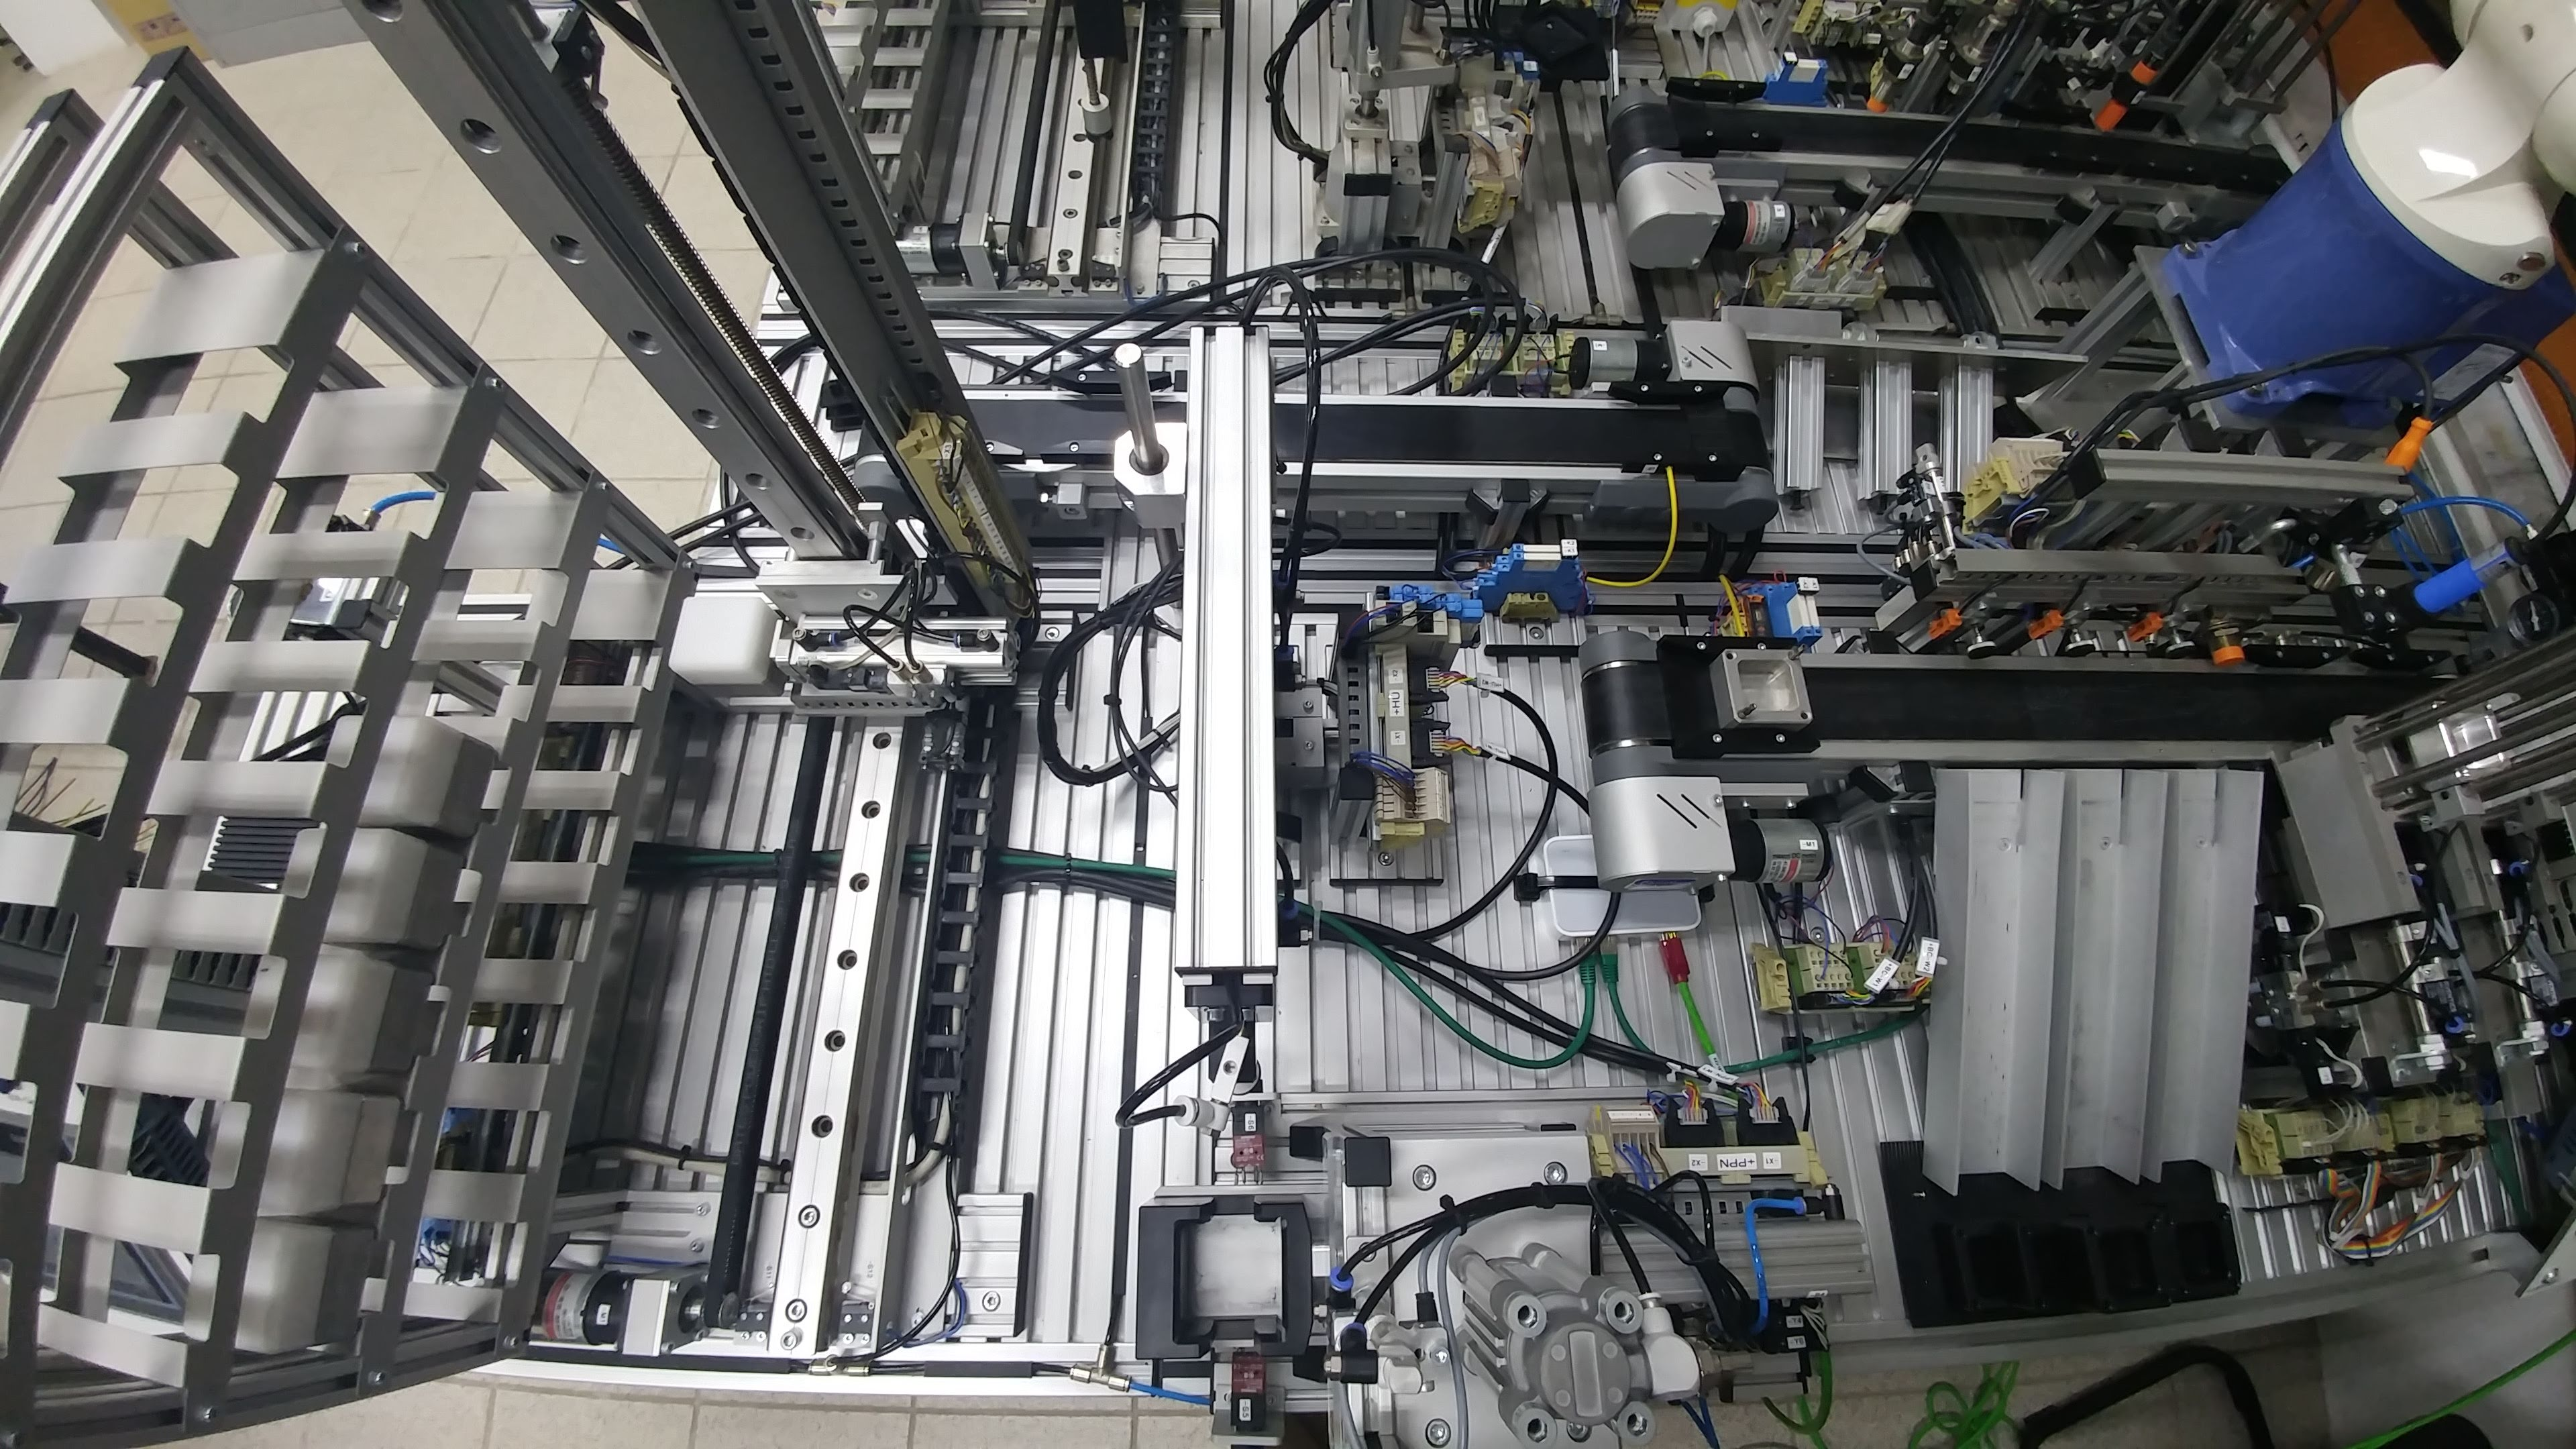
\includegraphics[trim={20cm 0 30cm 20cm},clip,width=0.8\textwidth]{maquete/armAngles.jpg}
    };
    % \draw[red,ultra thick,rounded corners] (0,0) rectangle (9.4,6.2);
    \begin{scope}[x={(image.south east)},y={(image.north west)}]
        % \draw[help lines,xstep=.1,ystep=.1] (0,0) grid (1,1);
        % \foreach \x in {0,1,...,9} { \node [anchor=north] at (\x/10,0) {0.\x}; }
        % \foreach \y in {0,1,...,9} { \node [anchor=east] at (0,\y/10) {0.\y}; }a
        
      
        \draw[red,->,>=stealth,very thick] (0.48,0.9) -- ++(-50:0.7);
        \draw[red,->,>=stealth,very thick] (0.48,0.9) -- ++(-95:0.7);
        \draw[red,->,>=stealth,very thick] (0.48,0.9) -- ++(-120:0.7);

        \draw[fill=red, fill opacity=0.2,draw=none] (0.48,0.9) -- ([shift=(-50:0.5)]0.48,0.9) arc (-50:-95:0.5);
        \draw[fill=blue, fill opacity=0.2,draw=none] (0.48,0.9) -- ([shift=(-95:0.5)]0.48,0.9) arc (-95:-120:0.5);

        \draw [fill,white,fill opacity=0.7,draw=none] (0.02,0.23) rectangle ++ (0.35,0.06);
        \draw [black] (0.2,0.25) node {\tiny \textbf{STORAGE\_ANGLE\_BEFORE}};

        \draw [fill,white,fill opacity=0.7,draw=none] (0.25,0.13) rectangle ++ (0.3,0.06);
        \draw [black] (0.4,0.15) node {\tiny \textbf{PRESS\_ANGLE\_AFTER}};

        \draw [fill,white,fill opacity=0.7,draw=none] (0.7,0.28) rectangle ++ (0.3,0.06);
        \draw [black] (0.85,0.3) node {\tiny \textbf{PRESS\_ANGLE\_BEFORE}};

        \draw [fill,white,fill opacity=0.7,draw=none] (0.1,0.82) rectangle  (0.2,0.96);
        \draw [red,thick] ([shift=(0:0.03)]0.15,0.9) arc (0:180:0.03);
        \draw[black,->,>=stealth,very thick] (0.15,0.85) -- ++(0,0.1);
        \draw [red,->,>=stealth,thick] ([shift=(0:-0.03)]0.15,0.9) arc (-180:-20:0.03);

      \end{scope}
  \end{tikzpicture}
  \caption{Arm Stop Logic Angles}
  \label{fig:armStopLogicAngles}
\end{figure}

The corresponding Petri net and tables can be seen in
\Autoref{fig:petriStorePiece} and
\Autoref{tab:storePieceTransitions,tab:storePiecePlaces}.
\newline
\begin{table}[H]
\caption{Arm Stop Logic Module Transitions.}
\centering
\begin{tabular}{M{5cm}M{10cm}}
Transitions & Meaning\\
\hline
\hyperlink{partialNet:t1561}{\hypertarget{partialTable:t156}{$t_{156}$}} & Stop Button\\
\hyperlink{partialNet:t1571}{\hypertarget{partialTable:t157}{$t_{157}$}} & ARMCOUNTER < STORAGE\(_{\text{ANGLE}}\)\(_{\text{BEFORE}}\)\\
\hyperlink{partialNet:t1581}{\hypertarget{partialTable:t158}{$t_{158}$}} & Arm Raised and Extended\\
\hyperlink{partialNet:t1591}{\hypertarget{partialTable:t159}{$t_{159}$}} & ARMCOUNTER >= STORAGE\(_{\text{ANGLE}}\)\(_{\text{BEFORE}}\)\\
\hyperlink{partialNet:t1601}{\hypertarget{partialTable:t160}{$t_{160}$}} & (ARMCOUNTER >= STORAGE\(_{\text{ANGLE}}\)\(_{\text{BEFORE}}\) and ARMCOUNTER < PRESS\(_{\text{ANGLE}}\)\(_{\text{AFTER}}\)) or ARMCOUNTER >= PRESS\(_{\text{ANGLE}}\)\(_{\text{BEFORE}}\)\\
\hyperlink{partialNet:t1611}{\hypertarget{partialTable:t161}{$t_{161}$}} & Arm Raised and Retracted\\
\hyperlink{partialNet:t1621}{\hypertarget{partialTable:t162}{$t_{162}$}} & Inductive Sensor Arm\\
\hyperlink{partialNet:t1631}{\hypertarget{partialTable:t163}{$t_{163}$}} & ARMCOUNTER >= PRESS\(_{\text{ANGLE}}\)\(_{\text{AFTER}}\) and ARMCOUNTER < PRESS\(_{\text{ANGLE}}\)\(_{\text{BEFORE}}\)\\
\hyperlink{partialNet:t1641}{\hypertarget{partialTable:t164}{$t_{164}$}} & Arm Retracted\\
\hyperlink{partialNet:t1651}{\hypertarget{partialTable:t165}{$t_{165}$}} & \(\overline{\mbox{Arm Retracted }}\)\\
\end{tabular}
\end{table}

\begin{longtable}{M{5cm}M{10cm}}
\caption{Arm Stop Logic Module Places.} \label{tab:armStopLogicPlaces}
\\
Places & Meaning\\
\hline
\endfirsthead
\multicolumn{2}{l}{Continued from previous page} \\
\hline

Places & Meaning \\

\hline
\endhead
\hline\multicolumn{2}{r}{Continued on next page} \\
\endfoot
\endlastfoot
\hline
\hyperlink{partialNet:p141}{\hypertarget{partialTable:p141}{$p_{141}$}} & \\
\hyperlink{partialNet:p142}{\hypertarget{partialTable:p142}{$p_{142}$}} & Raise and Extend Arm\\
\hyperlink{partialNet:p143}{\hypertarget{partialTable:p143}{$p_{143}$}} & Raise, Extend Arm and Turn CCW\\
\hyperlink{partialNet:p144}{\hypertarget{partialTable:p144}{$p_{144}$}} & Raise Arm\\
\hyperlink{partialNet:p145}{\hypertarget{partialTable:p145}{$p_{145}$}} & Raise Arm and Turn CCW\\
\hyperlink{partialNet:p146}{\hypertarget{partialTable:p146}{$p_{146}$}} & \\
\end{longtable}

\addtikzfigureLandscape{../../figures/petriNet/partial/armStopLogic}
{Petri net of manipulator Stop Logic module.}
{petriarmStopLogic}

\section{Implementation of the Control}
As said in other chapters, the implementation of the control in this work be implemented using \PLCs{}. The units shown in \Autoref{cha:system} were
divided in two parts and each part was connected to a Siemens \PLC{} S7-1500, as
the one shown in \Autoref{fig:plc}.

\begin{figure}[H]
\centering
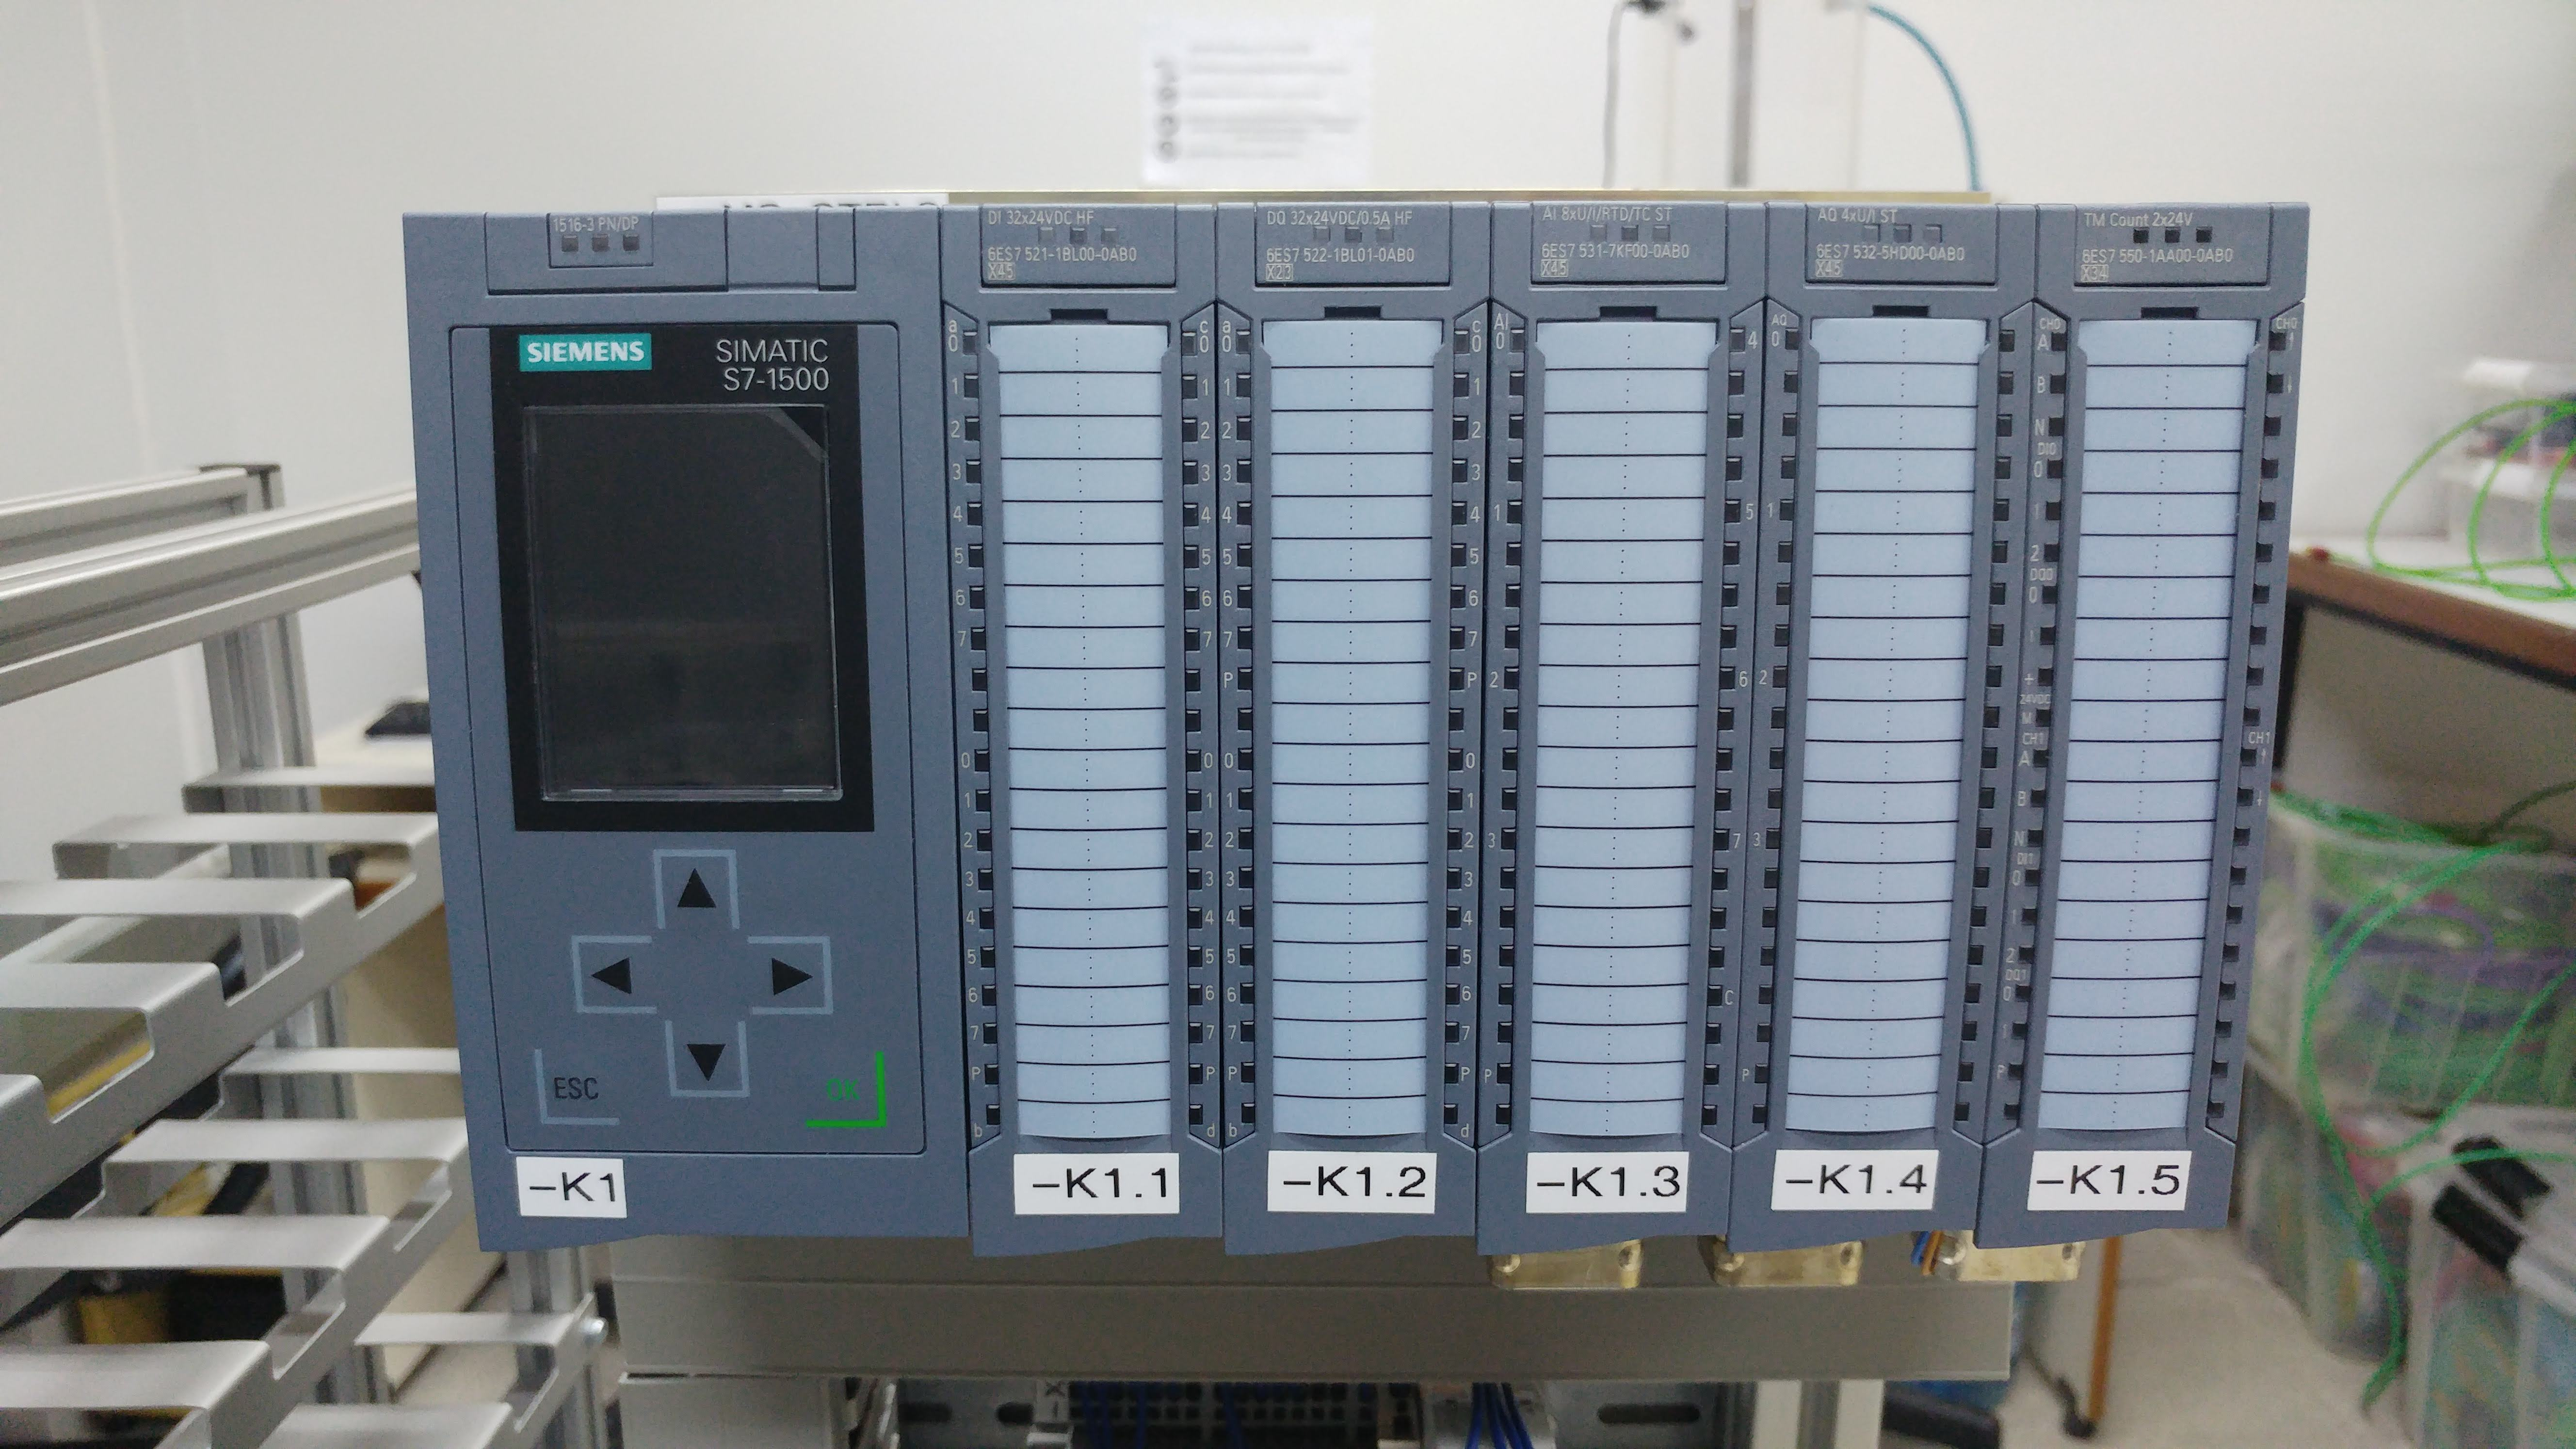
\includegraphics[width=0.7\textwidth,clip,trim={25cm 12cm 15cm 10cm}]{maquete/plc.jpg} 
  \caption{s7-1500}
  \label{fig:plc}
\end{figure}

The first \PLC{} was connected with both magazines,the conveyor belt and the
sorting unit. As those units are used to select the kind of pieces, this \PLC{}
is identified as Selection. In order to program the Ladder logic it is needed to
create tags to represent every input and output, so in
\Autoref{tab:plcSelectionInput,tab:plcSelectionOutput} we can see the
correspondence between the name of the input\slash output, the address in which
it is connected and the name of the tag created to represent it in the Ladder
Logic.

\begin{longtable}{c|c|c}
\caption{Inputs Selection PLC} \label{tab:plcSelectionInput}
\\
Input & Address & Tag\\
\hline
\endfirsthead
\multicolumn{3}{l}{Continued from previous page} \\
\hline

Input & Address & Tag \\

\hline
\endhead
\hline\multicolumn{3}{r}{Continued on next page} \\
\endfoot
\endlastfoot
\hline
MAG 1 Cylinder Extended & I0.0 & I\_MAG1EXT\\
MAG 1 Cylinder Retracted & I0.1 & I\_MAG1RET \\
MAG 1 Empty & I0.2 & I\_MAG1EMPT\\
MAG 2 Cylinder Extended & I0.3 & I\_MAG2EXT \\
MAG 2 Cylinder Retracted & I0.4 & I\_MAG2RET \\
MAG 2 Empty & I0.5 & I\_MAG2EMPT\\
Proximity Sensor Left Discharge Cylinder & I2.0 & I\_PSLD\\
Proximity Sensor Center Discharge Cylinder & I2.1 & I\_PSCD\\
Proximity Sensor Right Discharge Cylinder & I2.2 & I\_PSRD\\
Relay & I2.3 & I\_RELAY1\\
Left Discharge Cylinder Extended & I1.0 & I\_LDCEXT\\
Left Discharge Cylinder Retracted & I1.1 & I\_LDCRET\\
Center Discharge Cylinder Extended & I1.2 & I\_CDCEXT\\
Center Discharge Cylinder Retracted & I1.3 & I\_CDCRET\\
Right Discharge Cylinder Extended & I1.4 & I\_RDCEXT\\
Right Discharge Cylinder Retracted & I1.5 & I\_RDCRET\\
White Color Sensor & I1.6 & I\_WHIT\\
Metallic Sensor & I1.7 & I\_METAL\\
Proximity Sensor End Of Conveyor Belt & I0.6 & I\_PSEOC\\
Distance Sensor & IW4 & I\_DS\\
\end{longtable}

\begin{longtable}{c|c|c}
\caption{Outputs Selection PLC} \label{tab:plcSelectionOutput}
\\
Output & Address & Tag\\
\hline
\endfirsthead
\multicolumn{3}{l}{Continued from previous page} \\
\hline

Output & Address & Tag \\

\hline
\endhead
\hline\multicolumn{3}{r}{Continued on next page} \\
\endfoot
\endlastfoot
\hline
Extend MAG 1 Cylinder & Q1.0 & O\_MAG1EXT\\
Retract MAG 1 Cylinder & Q1.1 & O\_MAG1RET\\
Extend MAG 2 Cylinder & Q1.2 & O\_MAG2EXT\\
Retract MAG 2 Cylinder & Q1.3 & O\_MAG2RET\\
Extend Right Discharge Cylinder & Q0.2 & O\_RDCEXT\\
Extend Center Discharge Cylinder & Q0.1 & O\_CDCEXT\\
Extend Left Discharge Cylinder & Q0.0 & O\_LDCEXT\\
Conveyor Belt Forward & Q1.4 & O\_CBFW\\
Conveyor Belt Reverse & Q1.5 & O\_CBREV\\
\end{longtable}

As said in \Autoref{cha:system}, the \verb|Distance Sensor| outputs an integer
so the variables \verb|ConcUP| and \verb|ConcDWN| were created using the
following comparisons:
  \begin{align}
  \label{eq:concUpconcDown}
    % \verb|ConcUP|=2
    \text{\tt ConcUP} &=\text{\tt Distance Sensor} > \warning{values}\\
    \text{\tt ConcDWN}&=\text{\tt Distance Sensor} \leq \warning{values}
  \end{align}

The other units (Handling Unit, Assembly Unit and Storage Unit) are connected to
the second plc, identified as Handling-Assembly-Storage. The
\Autoref{tab:plcHandlingInput,tab:plcHandlingOutput} identify the addresses and
tags for this PLC.  
 
\begin{longtable}{c|c|c}
\caption{Inputs Handling-Assembly-Storage PLC} \label{tab:plcHandlingInput}
\\
Input & Address & Tag\\
\hline
\endfirsthead
\multicolumn{3}{l}{Continued from previous page} \\
\hline

Input & Address & Tag \\

\hline
\endhead
\hline\multicolumn{3}{r}{Continued on next page} \\
\endfoot
\endlastfoot
\hline
Safety Door Opened & I1.0 & I\_SDO      \\
Safety Door Closed & I1.1 & I\_SDC      \\
Assembly Unit Holder Extended & I1.2 & I\_AUHEXT   \\
Assembly Unit Holder Retracted & I1.3 & I\_AUHRET   \\
Inductive Sensor Arm & I0.2 & I\_INDARM   \\
Arm Lowered & I0.4 & I\_ARMLOW   \\
Arm Raised & I0.3 & I\_ARMHIG   \\
Arm Retracted & I0.6 & I\_ARMRET   \\
Arm Extended & I0.5 & I\_ARMEXT   \\
Storage Unit Vertical Encoder & I2.0 & I\_SUVE     \\
Storage Unit Inferior Limit Switch & I2.2 & I\_SUILS    \\
Storage Unit Superior Limit Switch & I2.1 & I\_SUSLS    \\
Storage Unit Extended & I2.3 & I\_SUEXT    \\
Storage Unit Retracted & I2.4 & I\_SURET    \\
Relay & I2.5 & I\_RELAY2   \\
Storage Unit Horizontal Encoder & I1.4 & I\_SUHE     \\
Storage Unit Right Limit Switch & I1.5 & I\_SURLS    \\
Storage Unit Left Limit Switch & I1.6 & I\_SULLS    \\
Storage Unit Arm Alignement Encoder & I1.7 & I\_SUARMALE \\
\end{longtable}

\begin{longtable}{c|c|c}
\caption{Outputs Handling-Assembly-Storage PLC} \label{tab:plcHandlingOutput}
\\
Output & Address & Tag\\
\hline
\endfirsthead
\multicolumn{3}{l}{Continued from previous page} \\
\hline

Output & Address & Tag \\

\hline
\endhead
\hline\multicolumn{3}{r}{Continued on next page} \\
\endfoot
\endlastfoot
\hline
Open Safety Door & Q0.6 & O\_SDO      \\
Close Safety Door & Q0.7 & O\_SDC      \\
Retract Assembly Unit Holder & Q1.1 & O\_AUHRET   \\
Extend Assembly Unit Holder & Q1.0 & O\_AUHEXT   \\
Lower Press & Q1.2 & O\_PRESSLOW \\
Raise Press & Q1.3 & O\_PRESSHIG \\
Raise Arm & Q0.0 & O\_ARMHIG   \\
Turn Vacuum Gripper ON & Q0.1 & O\_VACON    \\
Extend Arm & Q0.2 & O\_ARMEXT   \\
Turn Arm CCW & Q0.3 & O\_ARMCCW   \\
Turn Arm CW & Q0.4 & O\_ARMCW    \\
Extend Storage Unit & Q0.5 & O\_SUEXT    \\
Move Storage Unit Upwards & Q1.6 & O\_SUUP     \\
Move Storage Unit Downwards & Q1.7 & O\_SUDWN    \\
Move Storage Unit to the Right & Q1.5 & O\_SURIGHT  \\
Move Storage Unit to the Left & Q1.4 & O\_SULEFT   \\
\end{longtable}


To convert the \CIPN{} from the \Autoref{sec:logic} in to \LD{} the method
presented in \Autoref{sec:cipnToLD}. And in order to implement the connection
between the two \PLCs{} the method shown in \Autoref{sec:multiplePlcs} was used.
In order to configure the ``Get'' and ``Put'' blocks and consequentially the
connection between the two \PLCs, the tutorials shown in
section 3.4 of \cite{rochapereira2019automacao} was used.

For
brevity's sake the ladder logic was concealed, but can easily be
found at the following link
\url{https://github.com/Accacio/docsTCC/tree/master/PLC/TCC}, where all files of the TIA
Project used in this work is stored.




%%% Local Variables:
%%% mode: latex
%%% TeX-master: "../monografia"
%%% End:
